%
% $Header$
%

\documentclass[11pt]{article}

%\usepackage[dvips]{changebar}

\usepackage{subfigure}
\usepackage{fullpage}
\usepackage{setspace}         % XXX: enabling this may break the compilation
\usepackage{times}
\usepackage{latexsym}
\usepackage{psfig}
\usepackage{graphicx}
\usepackage{xspace}
\usepackage{color}
%\usepackage[dvipdf]{graphics}
%\usepackage[dvips]{graphicx}
%\usepackage{xorp}

\definecolor{gray}{rgb}{0.5,0.5,0.5}
\newcommand{\etc}{\emph{etc.}\xspace}
\newcommand{\ie}{\emph{i.e.,}\xspace}
\newcommand{\eg}{\emph{e.g.,}\xspace}
%\newcommand{\comment}[1]{{\color{gray}[\textsf{#1}]}}
\newcommand{\comment}[1]{}

% Changebar stuff
% \newenvironment{colorcode}{\color{blue}}{}
% \renewcommand{\cbstart}{\begin{colorcode}}
% \renewcommand{\cbend}{\end{colorcode}}

% \pagestyle{empty}

\begin{document}

\title{Using SNMP to manage XORP \\
\vspace{1ex}
Version 0.3}
\author{ XORP Project					\\
	 International Computer Science Institute	\\
	 Berkeley, CA 94704, USA			\\
	 {\it feedback@xorp.org}
}
\date{March 14, 2003}

\maketitle

\thispagestyle{empty}


%%%%%%%%%%%%%%%%%%%%%%%%%%%%%%%%%%%%%%%%%%%%%%%%%%%%%%%%%%%%%%%%%%%%%%%
\section{Introduction}


The SNMP standards \cite{snmp} define the protocol used to communicate between SNMP
managers and agents, as well as the structure of the management information
being accessed (MIB).  This document describes how XORP runtime data is made
accessible to the SNMP agent, how it is decomposed in separate MIB modules, and
how those modules are loaded/unloaded at runtime.  Also, a MIB development 
framework is presented, which provides unified process to those writing new MIB
modules for XORP.

%%%%%%%%%%%%%%%%%%%%%%%%%%%%%%%%%%%%%%%%%%%
\section{The SNMP agent}

XORP uses the extensible SNMP agent included in the Net-SNMP package \cite{net-snmp}.  
Net-SNMP provides tools and libraries supporting the Simple Network Management
Protocol.  The package is comprised of an extensible agent (\texttt{snmpd}), an SNMP
library and a set of command line tools to communicate with SNMP agents and
managers. 

Management information is viewed as a collection of managed objects, residing in
a virtual information store, termed the Management Information Base (MIB).  All
managed objects in the MIB are arranged in a hierarchical or tree structure.
Collections of related objects are defined in MIB modules.  These modules are
written in the SNMP data definition language, a subset of Abstract Syntax
Notation One (ASN.1).  New MIB modules that extend the Internet-standard MIB are
continuously being defined by various IETF working groups.  

In the context of this document, we'll extend the term MIB module to include the
part of the code that instantiates the objects declared in the MIB definition
file.  Thus a MIB module consists of:

\begin{description}
    \item[MIB module definition file] This file is written in ASN.1 language, and is
typically published as an RFC.
    \item[MIB module source code] One or more source files that implement the data
access routines that allow the SNMP agent to read or modify XORP's configuration settings. 
\end{description} 






%%%%%%%%%%%%%%%%%%%%%%%%%%%%%%%%%%%%%%%%%%%%%%%%%%%%%%%%%%%%%%%%%%%%%%%
\subsection{Dynamically loadable MIB modules}
\label{sec:MIB_module_format}

One of the guiding principles in XORP design is extensibility.  Protocols are
implemented as independent Unix processes that may come and go.  Each protocol
will have one or more associated MIB modules, so those modules should be made
available to the SNMP agent without requiring recompilation.  Net-SNMP supports
this strategy by allowing MIBs to be implemented as shared objects.  If your
system supports shared libraries, Net-SNMP will be compiled with support for
dynamically loadable MIB modules by default.  You can test if your Net-SNMP installation supports that option by looking for dlmod in the list printed by the command:

\begin{verbatim}
$ net-snmp-config --snmpd-module-list
\end{verbatim}


There are three methods for loading/unloading MIB modules:  

\begin{enumerate}
\item Using the dlmod directive in snmpd.conf 
\item Sending SNMP set requests to the agent
\item Using XORP's IPC methods (XRLs)
\end{enumerate}

The first option can only be used to load modules at startup.  This is what the man page for snmpd.conf tells you...

\begin{verbatim}
DYNAMICALLY LOADABLE MODULES
	If the agent is built with support for the UCD-DLMOD-MIB it is  capable
	of  loading  agent MIB modules dynamically at startup through the dlmod
	directive and during runtime through use  of  the  UCD-DLMOD-MIB.   The
	following directive loads the shared object module file PATH which uses
	the module name prefix NAME.

	dlmod NAME PATH
\end{verbatim}


To load MIBs using SNMP requests, a new row must be added to
UCD-DLMOD-MIB::dlmodTable.  This involves finding an unused index to the table,
setting the dlmodName and dlmodPath columns, and finally setting the column
dlmodStatus to 'load'.  These steps are captured in the following lines:

\begin{verbatim}
$ snmpwalk localhost UCD-DLMOD-MIB::dlmodTable
UCD-DLMOD-MIB::dlmodName.1 = STRING: xorp_if_mib_module
UCD-DLMOD-MIB::dlmodPath.1 = STRING: /scratch/xorp/mibs/xorp_if_mib_module.so
UCD-DLMOD-MIB::dlmodError.1 = STRING:
UCD-DLMOD-MIB::dlmodStatus.1 = INTEGER: loaded(1)

$ snmpset localhost UCD-DLMOD-MIB::dlmodStatus.2 i create
UCD-DLMOD-MIB::dlmodStatus.2 = INTEGER: create(6)


$ snmpset localhost UCD-DLMOD-MIB::dlmodName.2 s "bgp4_mib_1657" UCD-DLMOD-MIB::dlmodPath.2 s "/scratch/xorp/mibs/bgp4_mib_1657.so"
UCD-DLMOD-MIB::dlmodName.2 = STRING: bgp4_mib_1657
UCD-DLMOD-MIB::dlmodPath.2 = STRING: /scratch/xorp/mibs/bgp4_mib_1657.so

$ snmpset localhost UCD-DLMOD-MIB::dlmodStatus.2 i load
UCD-DLMOD-MIB::dlmodStatus.2 = INTEGER: load(4)

$ snmpwalk localhost UCD-DLMOD-MIB::dlmodTable
UCD-DLMOD-MIB::dlmodName.1 = STRING: xorp_if_mib_module
UCD-DLMOD-MIB::dlmodName.2 = STRING: bgp4_mib_1657
UCD-DLMOD-MIB::dlmodPath.1 = STRING: /scratch/xorp/mibs/xorp_if_mib_module.so
UCD-DLMOD-MIB::dlmodPath.2 = STRING: /scratch/xorp/mibs/bgp4_mib_1657.so
UCD-DLMOD-MIB::dlmodError.1 = STRING:
UCD-DLMOD-MIB::dlmodError.2 = STRING:
UCD-DLMOD-MIB::dlmodStatus.1 = INTEGER: loaded(1)
UCD-DLMOD-MIB::dlmodStatus.2 = INTEGER: loaded(1)
\end{verbatim}

We've seen so far how to load MIBs when the agent is started, and at runtime via SNMP requests.  But XORP processes communicate to each other via XRLs, and it would be quite inconvenient for a process to require sending SNMP requests whenever it needs to load or unload a MIB.  This is why we've implemented an Xrl target into Net-SNMP.  After the module \texttt{xorp\_if\_mib\_module} is loaded, Net-SNMP can accept XRL's.  In particular the following XRLs should be used for loading/unloading MIBs:

\begin{ttfamily}
\begin{verbatim}
finder://xorp_if_mib/xorp_if_mib/0.1/load_mib?mod_name:txt&abs_path:txt
finder://xorp_if_mib/xorp_if_mib/0.1/unload_mib?mib_index:u32
\end{verbatim}
\end{ttfamily}

Dynamically loadable MIB modules written for the main SNMP agent can also be
loaded by an SNMP sub-agent that communicates with the master agent via the
AgentX protocol (\ref{}).  This should be useful in the event that you
configure XORP to run distributed across multiple hosts but with one 
master SNMP agent.  


%%%%%%%%%%%%%%%%%%%%%%%%%%%%%%%%%%%%%%%%%%%
\section{Connecting Net-SNMP with XORP}


We have written a special MIB module (\texttt{xorp\_if\_mib\_module}) that
coordinates the communication between \texttt{snmpd} and XORP processes.  This
module provides several classes that allow XORP MIB modules to be architected
as if they were each executed as independent processes (although they all run
in \texttt{snmpd}'s process space).  This should make MIB module design much easier to someone already familiar with the arquitecture of XORP processes.
 
The class that does all the syncronization between XORP and Net-SNMP 
is SnmpEventLoop, a subclass of EventLoop.  This singleton class is
responsible for registering XORP event's with \texttt{snmpd}, so that the agent
can respond to XORP activity.  Once this class is instantiated by
\texttt{xorp\_if\_mib\_module}, it can be used by all the other MIB modules as
if it was their own EventLoop.  Without it, MIB modules could not respond to
XORP events, this is why this module must be loaded before any other, and
should be the last XORP MIB module to be unloaded \footnote{rtld}.  Typically you would use the snmpd.conf file to load it at start up time.  

The XORP interface MIB module also implements the XRL target (\cite{}) that
allows the loading and unloading of other MIB modules.  


Figure \ref{fig:xorp-if-diag} illustrates the functionality implemented by 
\texttt{xorp\_if\_mib\_module}.

\begin{figure}
  \begin{center}
    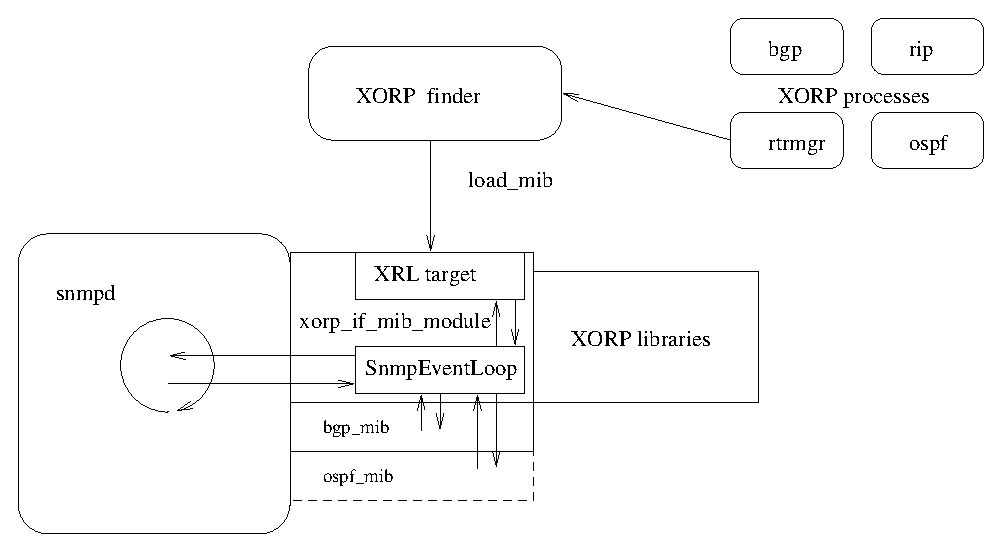
\includegraphics[width=1\textwidth]{figs/snmp_fig2}
  \end{center}
  \caption{Role of xorp\_if\_mib\_module}
  \label{fig:xorp-if-diag}
\end{figure}




\subsection{Modifying XORP's configuration}


MIB modules use XORP's IPC library \cite{xorp:xrl}.  Each MIB module has the
responsibility to pull the relevant management information from the appropriate
process (\eg BGP MIB data from BGP process).  For that effect, the MIB module
must implement the XRL Interface supported by the XRL targets it needs to
communicate to (see \cite{xorp:xrl_interfaces} for details on how to implement
XRL Interface Client classes).  MIB modules, though, MUST not modify any
configuration settings by accessing the process directly.  The current state of
configuration is maintained by the router manager process, so bypassing it would
cause the real and the recorded configurations to be out of sync.  Instead,
configuration changes should be requested to the router manager via
configuration commands, that is, XRLs such as the ones appearing in the template
files (see xorp/etc/templates/*.tp).

Figure \ref{fig:mib-class-diag} illustrates the architecture of MIB modules.
\begin{figure}
  \begin{center}
    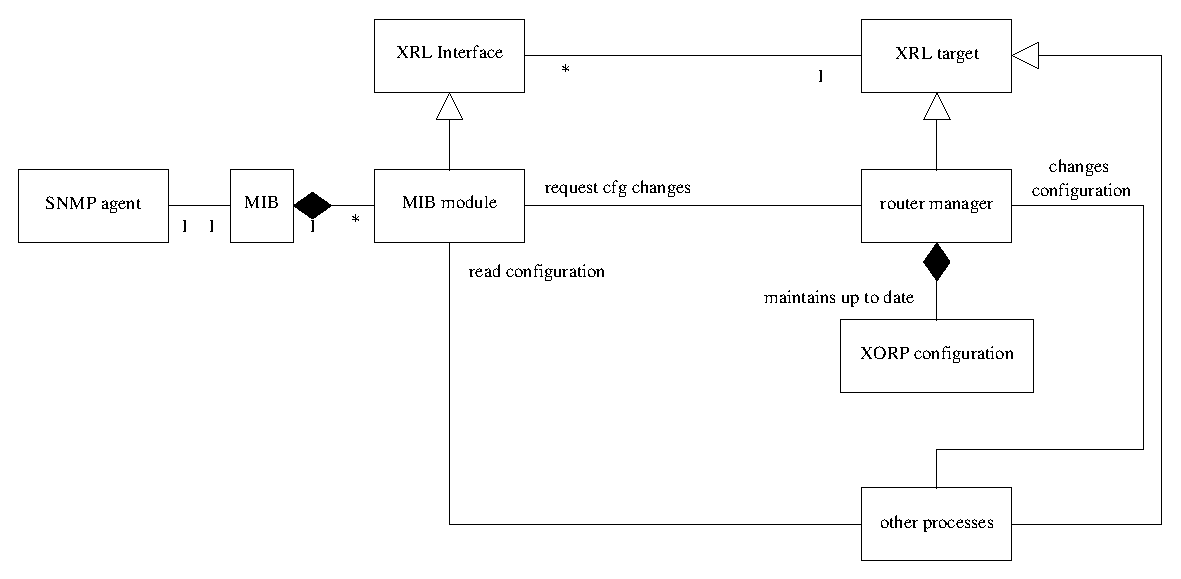
\includegraphics[width=1\textwidth]{figs/snmp_fig1}
  \end{center}
  \caption{Class diagram showing MIB modules interdependencies}
  \label{fig:mib-class-diag}
\end{figure}


%%%%%%%%%%%%%%%%%%%%%%%%%%%%%%%%%%%%%%%%%%%
\section{A reference implementation of a MIB module}

So far we've talked about Net-SNMP configuration.  In this section we'll cover how to write a MIB module.  

The first step should be writting or getting the ASN.1 MIB definition file.  If you are implementing an existing protocol, chances are that there is already a published RFC with the MIB definition for it.  In this release we have partially implemented the BGP4-MIB, which is published in RFC 1657.

\subsection{Using delegated requests}
\subsection{Using mib2c}
\subsection{Configuring the agent}
\subsection{Accessing the MIBS}

%%%%%%%%%%%%%%%%%%%%%%%%%%%%%%%%%%%%%%%%%%%%%%%%%%%%%%%%%%%%%%%%%%%%%%%
%     APPENDIX
%%%%%%%%%%%%%%%%%%%%%%%%%%%%%%%%%%%%%%%%%%%%%%%%%%%%%%%%%%%%%%%%%%%%%%%
\appendix
\section{Modification History}

\begin{itemize}

  \item March 14, 2003: Created.

\end{itemize}

%%%%%%%%%%%%%%%%%%%%%%%%%%%%%%%%%%%%%%%%%%%%%%%%%%%%%%%%%%%%%%%%%%%%%%%
%     BIBLIOGRAPHY
%%%%%%%%%%%%%%%%%%%%%%%%%%%%%%%%%%%%%%%%%%%%%%%%%%%%%%%%%%%%%%%%%%%%%%%
\bibliography{../tex/xorp}
\bibliographystyle{plain}

%%%%%%%%%%%%%%%%%%%%%%%%%%%%%%%%%%%%%%%%%%%%%%%%%%%%%%%%%%%%%%%%%%%%%%%
\end{document}
